\begin{figure}[H]
    \centering
    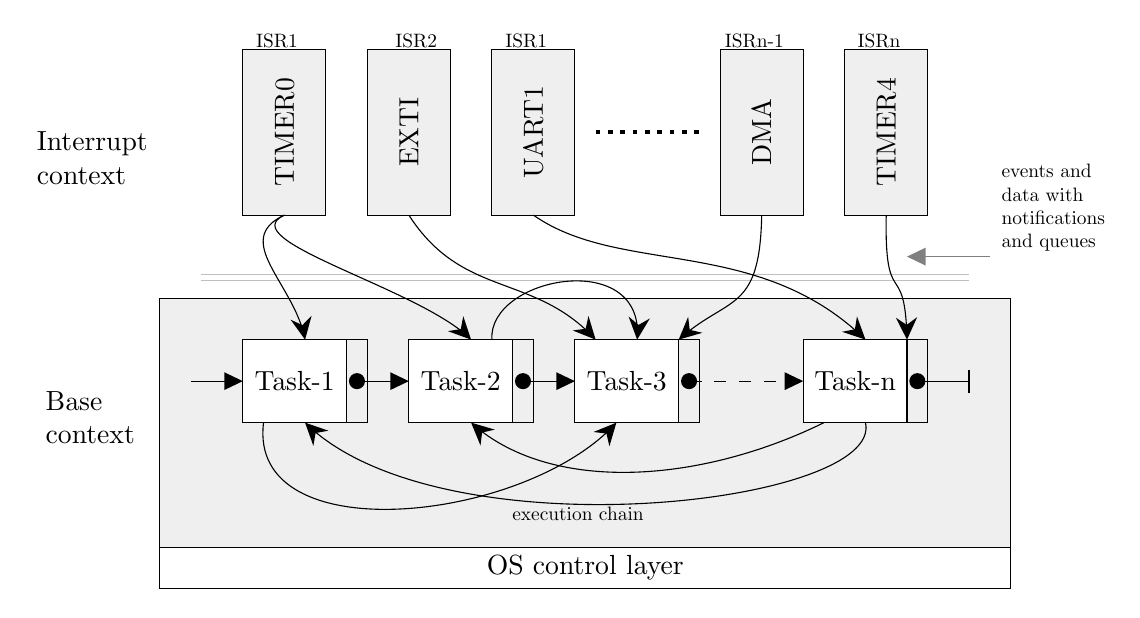
\begin{tikzpicture}[x=0.75pt,y=0.75pt,yscale=-1,xscale=1,scale=1]
        \draw  [fill=lightgray!25  ,fill opacity=1 ] (170,200) -- (580,200) -- (580,340) -- (170,340) -- cycle ;
        \draw  [fill=lightgray!25   ,fill opacity=1 ] (210,80) -- (250,80) -- (250,160) -- (210,160) -- cycle ;
        \draw  [fill=lightgray!25   ,fill opacity=1 ] (270,80) -- (310,80) -- (310,160) -- (270,160) -- cycle ;
        \draw  [fill=lightgray!25  ,fill opacity=1 ] (330,80) -- (370,80) -- (370,160) -- (330,160) -- cycle ;
        \draw  [fill=lightgray!25   ,fill opacity=1 ] (440,80) -- (480,80) -- (480,160) -- (440,160) -- cycle ;
        \draw  [fill=lightgray!25   ,fill opacity=1 ] (500,80) -- (540,80) -- (540,160) -- (500,160) -- cycle ;
        \draw [line width=1.5]  [dash pattern={on 1.69pt off 2.76pt}]  (380,120) -- (430,120) ;
        \draw  [fill=white  ,fill opacity=1 ] (210,220) -- (260,220) -- (260,260) -- (210,260) -- cycle ;
        \draw   (260,220) -- (270,220) -- (270,260) -- (260,260) -- cycle ;
        \draw  [fill=white  ,fill opacity=1 ] (290,220) -- (340,220) -- (340,260) -- (290,260) -- cycle ;
        \draw   (340,220) -- (350,220) -- (350,260) -- (340,260) -- cycle ;
        \draw  [fill=white  ,fill opacity=1 ] (370,220) -- (420,220) -- (420,260) -- (370,260) -- cycle ;
        \draw   (420,220) -- (430,220) -- (430,260) -- (420,260) -- cycle ;
        \draw  [fill=white  ,fill opacity=1 ] (480,220) -- (530,220) -- (530,260) -- (480,260) -- cycle ;
        \draw   (530,220) -- (540,220) -- (540,260) -- (530,260) -- cycle ;
        \draw    (265,240) -- (288,240) ;
        \draw [shift={(290,240)}, rotate = 180] [fill=black ][line width=0.75]  [draw opacity=0] (8.93,-4.29) -- (0,0) -- (8.93,4.29) -- cycle    ;
        \draw [shift={(265,240)}, rotate = 0] [color=black ][fill=black ][line width=0.75]      (0, 0) circle [x radius= 3.35, y radius= 3.35]   ;
        \draw    (345,240) -- (368,240) ;
        \draw [shift={(370,240)}, rotate = 180] [fill=black ][line width=0.75]  [draw opacity=0] (8.93,-4.29) -- (0,0) -- (8.93,4.29) -- cycle    ;
        \draw [shift={(345,240)}, rotate = 0] [color=black ][fill=black ][line width=0.75]      (0, 0) circle [x radius= 3.35, y radius= 3.35]   ;
        \draw    (535,240) -- (560,240) ;
        \draw [shift={(560,240)}, rotate = 180] [color=black ][line width=0.75]    (0,5.59) -- (0,-5.59)   ;
        \draw [shift={(535,240)}, rotate = 0] [color=black ][fill=black ][line width=0.75]      (0, 0) circle [x radius= 3.35, y radius= 3.35]   ;
        \draw  [dash pattern={on 4.5pt off 4.5pt}]  (425,240) -- (478,240) ;
        \draw [shift={(480,240)}, rotate = 180] [fill=black ][line width=0.75]  [draw opacity=0] (8.93,-4.29) -- (0,0) -- (8.93,4.29) -- cycle    ;
        \draw [shift={(425,240)}, rotate = 0] [color=black ][fill=black ][line width=0.75]      (0, 0) circle [x radius= 3.35, y radius= 3.35]   ;
        \draw    (185,240) -- (208,240) ;
        \draw [shift={(210,240)}, rotate = 180] [fill=black ][line width=0.75]  [draw opacity=0] (8.93,-4.29) -- (0,0) -- (8.93,4.29) -- cycle    ;
        \draw [color=lightgray  ,draw opacity=1 ]   (190,188.5) -- (560,188.5)(190,191.5) -- (560,191.5) ;
        \draw    (230,160) .. controls (204.63,171.97) and (233.89,192.37) .. (239.68,218.4) ;
        \draw [shift={(240,220)}, rotate = 259.65] [fill=black ][line width=0.75]  [draw opacity=0] (10.72,-5.15) -- (0,0) -- (10.72,5.15) -- (7.12,0) -- cycle    ;
        \draw    (230,160) .. controls (204.5,172.03) and (293.37,194.79) .. (318.88,218.9) ;
        \draw [shift={(320,220)}, rotate = 225.74] [fill=black ][line width=0.75]  [draw opacity=0] (10.72,-5.15) -- (0,0) -- (10.72,5.15) -- (7.12,0) -- cycle    ;
        \draw    (330,220) .. controls (328.14,190.03) and (401.85,176) .. (400.13,218.04) ;
        \draw [shift={(400,220)}, rotate = 275.28] [fill=black ][line width=0.75]  [draw opacity=0] (10.72,-5.15) -- (0,0) -- (10.72,5.15) -- (7.12,0) -- cycle    ;
        \draw    (510,260) .. controls (519.06,299.2) and (307.24,324.14) .. (240.99,260.96) ;
        \draw [shift={(240,260)}, rotate = 404.68] [fill=black ][line width=0.75]  [draw opacity=0] (10.72,-5.15) -- (0,0) -- (10.72,5.15) -- (7.12,0) -- cycle    ;
        \draw    (350,160) .. controls (391.9,189.34) and (457.45,169.68) .. (509.22,219.25) ;
        \draw [shift={(510,220)}, rotate = 224.23] [fill=black ][line width=0.75]  [draw opacity=0] (10.72,-5.15) -- (0,0) -- (10.72,5.15) -- (7.12,0) -- cycle    ;
        \draw    (460,160) .. controls (459.13,206.53) and (444.7,198.82) .. (421.44,218.74) ;
        \draw [shift={(420,220)}, rotate = 318.25] [fill=black ][line width=0.75]  [draw opacity=0] (10.72,-5.15) -- (0,0) -- (10.72,5.15) -- (7.12,0) -- cycle    ;
        \draw    (220,260) .. controls (212.19,321.86) and (343.44,308.76) .. (388.66,261.44) ;
        \draw [shift={(390,260)}, rotate = 492.15] [fill=black ][line width=0.75]  [draw opacity=0] (10.72,-5.15) -- (0,0) -- (10.72,5.15) -- (7.12,0) -- cycle    ;
        \draw    (290,160) .. controls (315.72,199.88) and (349.09,187.86) .. (378.65,218.57) ;
        \draw [shift={(380,220)}, rotate = 227.41] [fill=black ][line width=0.75]  [draw opacity=0] (10.72,-5.15) -- (0,0) -- (10.72,5.15) -- (7.12,0) -- cycle    ;
        \draw  [fill=white  ,fill opacity=1 ] (170,320) -- (580,320) -- (580,340) -- (170,340) -- cycle ;
        \draw    (520,160) .. controls (519.12,206.77) and (528.81,180.22) .. (529.95,218.22) ;
        \draw [shift={(530,220)}, rotate = 268.74] [fill=black ][line width=0.75]  [draw opacity=0] (10.72,-5.15) -- (0,0) -- (10.72,5.15) -- (7.12,0) -- cycle    ;
        \draw [color=gray  ,draw opacity=1 ]   (570,180) -- (532,180) ;
        \draw [shift={(530,180)}, rotate = 360] [fill=gray  ,fill opacity=1 ][line width=0.75]  [draw opacity=0] (8.93,-4.29) -- (0,0) -- (8.93,4.29) -- cycle    ;
        \draw    (490,260) .. controls (430.71,289.1) and (359.55,294.29) .. (321.15,261.02) ;
        \draw [shift={(320,260)}, rotate = 402.07] [fill=black ][line width=0.75]  [draw opacity=0] (10.72,-5.15) -- (0,0) -- (10.72,5.15) -- (7.12,0) -- cycle    ;
        \draw (230,120) node [rotate=-270] [align=left] {TIMER0};
        \draw (290,120) node [rotate=-270] [align=left] {EXTI};
        \draw (350,120) node [rotate=-270] [align=left] {UART1};
        \draw (460,120) node [rotate=-270] [align=left] {DMA};
        \draw (520,120) node [rotate=-270] [align=left] {TIMER4};
        \draw (235,240) node  [align=left] {Task-1};
        \draw (315,240) node  [align=left] {Task-2};
        \draw (395,240) node  [align=left] {Task-3};
        \draw (505,240) node  [align=left] {Task-n};
        \draw (226.5,76) node [scale=0.7] [align=left] {ISR1};
        \draw (293.5,76) node [scale=0.7] [align=left] {ISR2};
        \draw (346.5,76) node [scale=0.7] [align=left] {ISR1};
        \draw (516.5,76) node [scale=0.7] [align=left] {ISRn};
        \draw (456.5,76) node [scale=0.7] [align=left] {ISRn-1};
        \draw (136.5,257.5) node  [align=left] {Base \\context};
        \draw (137.5,132.5) node  [align=left] {Interrupt \\context};
        \draw (375,330) node  [align=left] {OS control layer};
        \draw (371.5,304) node [scale=0.7] [align=left] {execution chain};
        \draw (600.5,156.5) node [scale=0.7] [align=left] {events and\\data with\\notifications\\and queues};
    \end{tikzpicture}
    \caption{Heavy cooperative environment}
    \label{fig:heavyenvy}
\end{figure}